\documentclass[tikz,border=0pt]{standalone}
\usepackage{xcolor}
\usetikzlibrary{calc}
% Palette: Sam_Comm_final.png by eye (vagrancy repository).
\definecolor{ink}{HTML}{3B2340}
\definecolor{dark}{HTML}{4A3357}
\definecolor{darkhi}{HTML}{5E4A6E}
\definecolor{sky}{HTML}{EFC46A}
\definecolor{skyhi}{HTML}{F5DA92}
\definecolor{skylow}{HTML}{E9B060}
\definecolor{cloud}{HTML}{F2D58A}
\definecolor{wallA}{HTML}{E88A73}
\definecolor{wallB}{HTML}{EE9F7E}
\definecolor{wallC}{HTML}{E47A7E}
\definecolor{wallD}{HTML}{F0B07E}
\definecolor{wallE}{HTML}{D9765F}
\definecolor{wallF}{HTML}{E99A8A}
\definecolor{greenA}{HTML}{8DBB7E}
\definecolor{greenB}{HTML}{6FA77A}
\definecolor{greenC}{HTML}{A9C97F}
\definecolor{greenD}{HTML}{5E9C6A}
\definecolor{window}{HTML}{F6E7A0}
\definecolor{windark}{HTML}{8C5A64}
\definecolor{plum}{HTML}{8A5A9E}
\definecolor{plumhi}{HTML}{A77BB8}
\definecolor{lilac}{HTML}{D9C3E0}
\definecolor{coral}{HTML}{E47A7E}
\definecolor{coraldk}{HTML}{C85F65}
\definecolor{orange}{HTML}{F26B38}
\definecolor{salmon}{HTML}{F4BE9C}
\definecolor{gold}{HTML}{F2B53A}
\definecolor{golddk}{HTML}{D9962A}
\definecolor{butter}{HTML}{F5DA92}
\definecolor{cream}{HTML}{FFF4E0}
\definecolor{paper}{HTML}{F6E7C4}
\definecolor{sage}{HTML}{8DBB7E}
\definecolor{sagedk}{HTML}{6FA77A}
\definecolor{forest}{HTML}{5E9C6A}
\definecolor{mint}{HTML}{C5E0B4}
\definecolor{teal}{HTML}{5FA8A0}
\definecolor{glass}{HTML}{A9D3C9}
\definecolor{glassdk}{HTML}{7FB7B0}
\definecolor{pink}{HTML}{F2A7B5}
\definecolor{rosewall}{HTML}{F3B7A8}
\definecolor{steel}{HTML}{C8C2B4}
\definecolor{steeldk}{HTML}{8D9A93}
\definecolor{metal}{HTML}{8D9A93}
\definecolor{wood}{HTML}{B9835A}
\definecolor{wooddk}{HTML}{8E5E3C}
\definecolor{tan}{HTML}{E2BD8C}
\definecolor{paving}{HTML}{E2BD8C}
\definecolor{ground}{HTML}{D3A77D}
% One ink for every outline.
\newcommand{\Ink}{1.3pt}
\tikzset{inked/.style={draw=ink, line width=\Ink, line join=round, line cap=round}}
% Picture units: 0.4 mm, y counted downward (hence the negative y unit).
\tikzset{x=0.4mm, y=-0.4mm}
\begin{document}
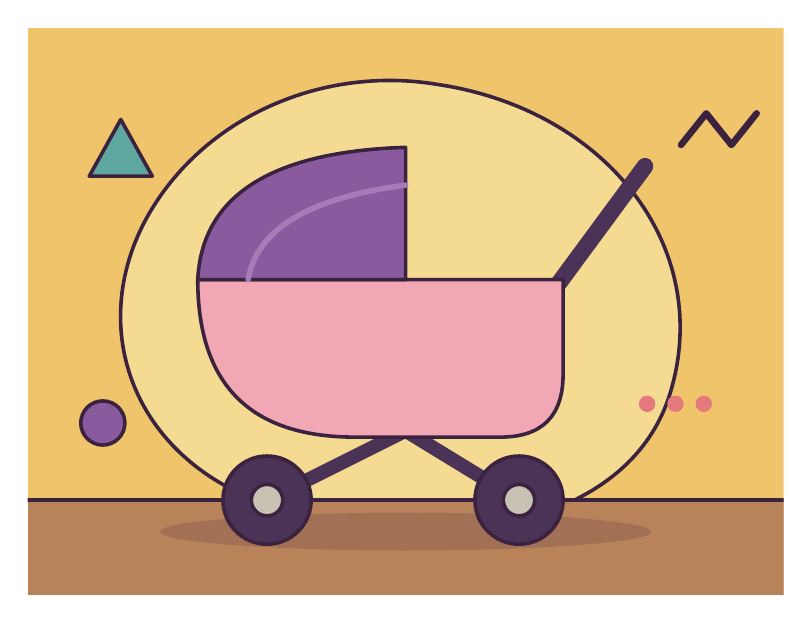
\begin{tikzpicture}
\clip (0,0) rectangle (240,180);
% background: wall, floor, blob, confetti
\fill[sky] (0,0) rectangle (240,180);
\filldraw[inked,fill=skyhi] (130,18) .. controls (184,26) and (218,70) .. (204,116) .. controls (190,162) and (122,168) .. (78,152) .. controls (34,138) and (18,96) .. (38,60) .. controls (56,28) and (94,12) .. (130,18) -- cycle;
\filldraw[inked,fill=plum] (23.86,125.51) circle [radius=7];
\draw[ink, line width=2.4pt, line cap=round, line join=round] (207.45,37.22) -- (215.45,27.22) -- (223.45,37.22) -- (231.45,27.22);
\filldraw[inked,fill=teal] (19.56,47.15) -- (29.56,29.15) -- (39.56,47.15) -- cycle;
\foreach \dx in {0,9,18} \fill[coral] (196.67+\dx,119.42) circle [radius=2.6];
\fill[wood] (0,150) rectangle (240,180);
\draw[ink, line width=1.3pt, line cap=round, line join=round] (0,150) -- (240,150);
\fill[ink, opacity=0.18] (120,160) ellipse [x radius=78, y radius=6];
% the item
\draw[dark, line width=5pt, line cap=round, line join=round] (76,150) -- (120,128) -- (156,150);
\draw[dark, line width=6pt, line cap=round, line join=round] (168,82) -- (196,44);
\filldraw[inked,fill=pink] (54,80) .. controls (54,113.33) and (70.67,130) .. (104,130) -- (150,130) .. controls (163.33,130) and (170,123.33) .. (170,110) -- (170,80) -- cycle;
\filldraw[inked,fill=plum] (54,80) .. controls (55.33,53.33) and (77.33,39.33) .. (120,38) -- (120,80) -- cycle;
\draw[plumhi, line width=2pt, line cap=round, line join=round] (70,80) .. controls (72.67,64) and (89.33,54) .. (120,50);
\filldraw[inked,fill=dark] (76,150) circle [radius=14];
\filldraw[inked,fill=steel] (76,150) circle [radius=5];
\filldraw[inked,fill=dark] (156,150) circle [radius=14];
\filldraw[inked,fill=steel] (156,150) circle [radius=5];
\end{tikzpicture}
\end{document}
